
\section{Problem Formulation}
\label{sec:form}

We formulate the problem in following way

\subsection{Runtime Exceptions}
\label{subsec:excep}

\begin{figure}[htb]
\centering
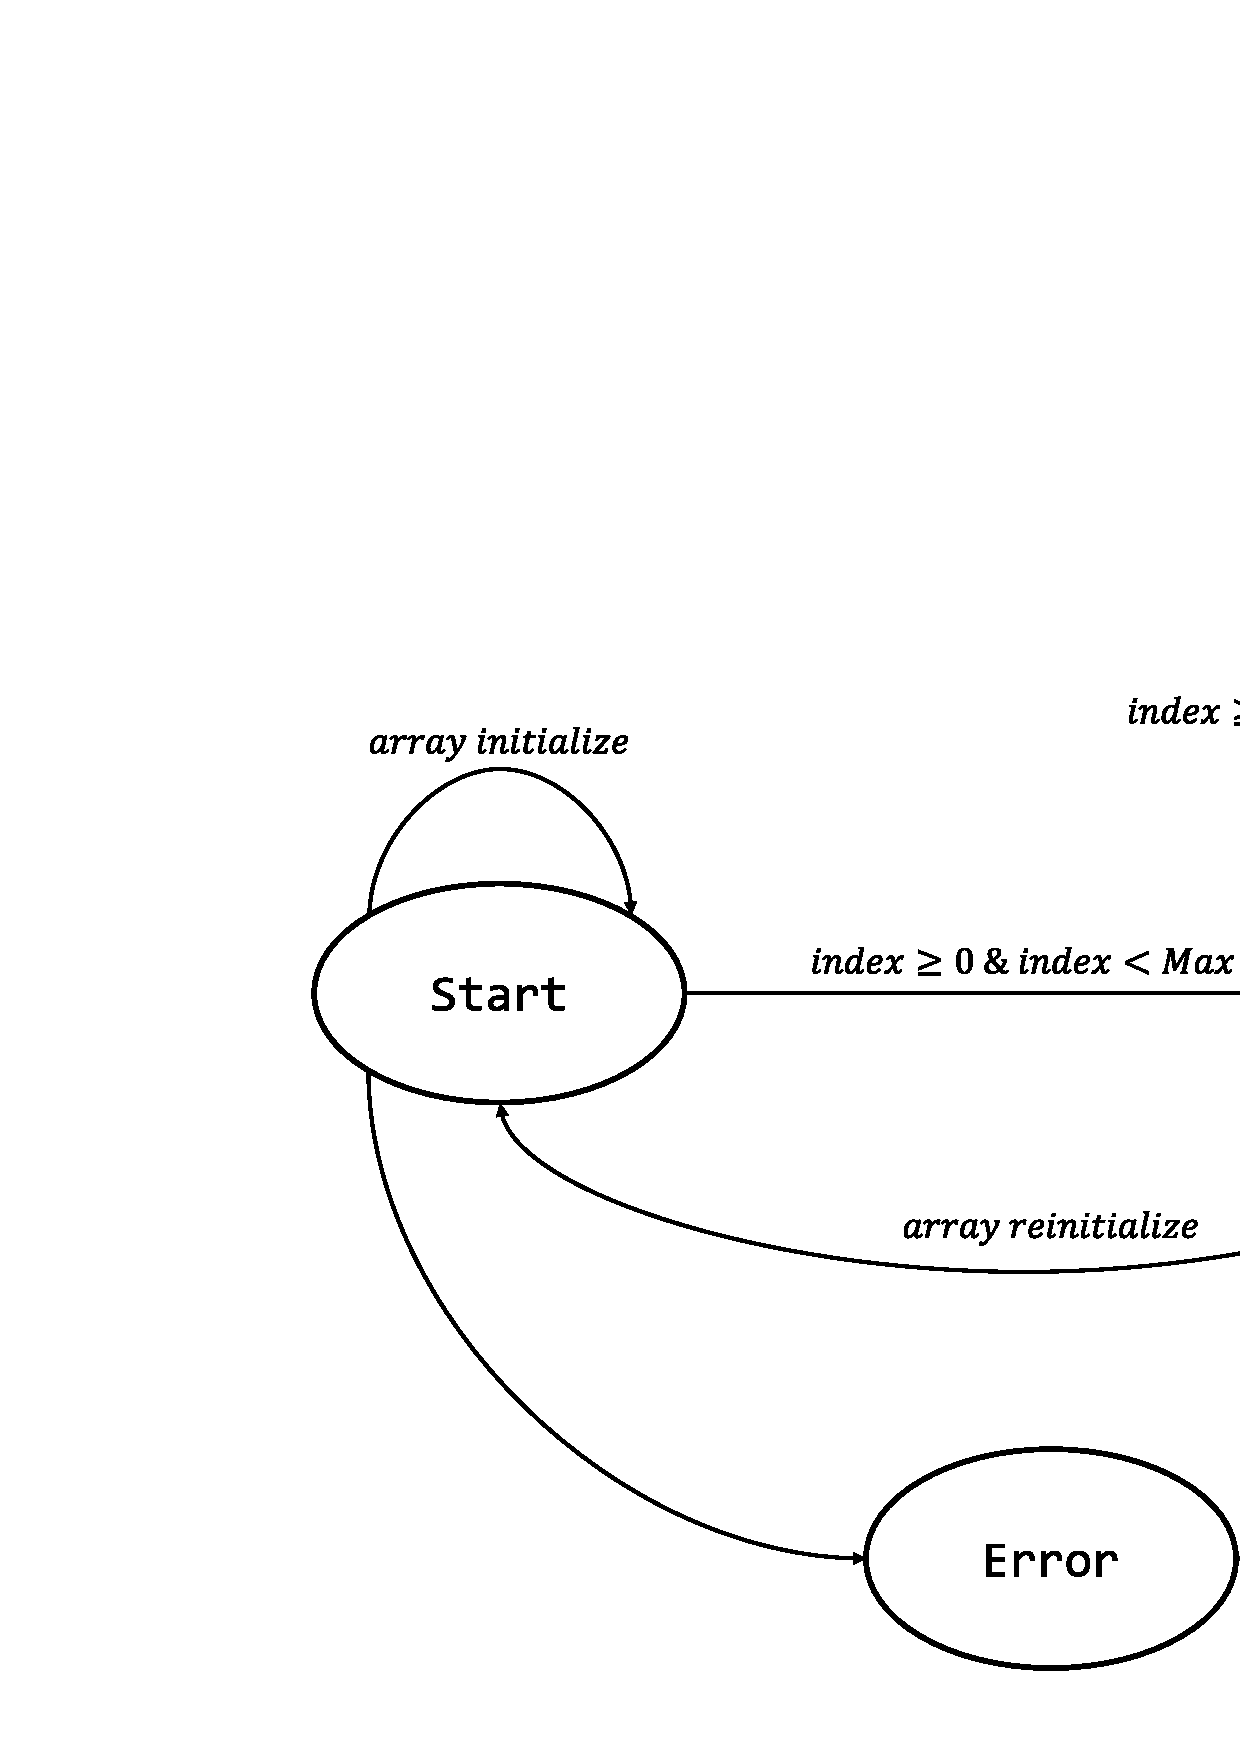
\includegraphics[scale = .25]{images/ArrayIndex.pdf}
\caption{array index out of bound formulated as FSM}
\label{fig:array}
\end{figure}


We can visualize all runtime exceptions as finite state machine (FSM). When a
program violates such sequence, it throws runtime exception. 
In Figure~\ref{fig:array}, array index out of bound (java.lang.
ArrayIndexOutOfBoundException) exception is described as a FSM. 
Here, a program will be in safe bound as long as the $array\_index \geq 0$ or
$array\_index \leq max\_array\_size - 1$

\subsection{Constraint Automata}
\label{subsec:constraintAutomata}

\emph{Constraint automata} is a formalism to describe the behavior and possible
data flow in coordination models. 
Mostly used for model checking. We have used it for the purpose of program
repairing technique. Here we define the finite state automata as follows :

$$(Q, \Sigma, \delta, q_0, F)$$
\begin{mybullet}
 \item $Q$: set of state where $|Q| = 2$, \emph{legal state}(init) and
\emph{illegal state} (error).
 \item $\Sigma$: symbols, invariants based on exception type.
 \item $\delta$: transition function. $init \rightarrow init$ is safe
transition and $init \rightarrow error$ is the invariant violation.
 \item $q_0$: starting state, here $q_0 = init$.
 \item $F$: end state, here it same as $q_0$.
\end{mybullet}

\begin{figure}[t]
\centering
\includegraphics[scale=.25]{images/automata.pdf}
\caption{Constraint automata general model}
\label{fig:automata}
\end{figure}

According to the Figure~\ref{fig:automata}, the repairing mechanism will only
trigger when we have a transition from 
init state to error state due to invariant violation.

\subsection{Patching Techniques}
\label{subsec:patchCA}

The patching technique is based on the exception type. 
